%----------------------------------------------------------------------------------------
%	PACKAGES AND OTHER DOCUMENT CONFIGURATIONS
%----------------------------------------------------------------------------------------

\documentclass[12pt]{article} % Font size (can be 10pt, 11pt or 12pt) and paper size (remove a4paper for US letter paper)

\usepackage[protrusion=true,expansion=true]{microtype} % Better typography
\usepackage{graphicx} % Required for including pictures
\usepackage{wrapfig} % Allows in-line images
\usepackage{amsmath}
\usepackage{xfrac}
\usepackage{mathtools}
\usepackage{geometry}
\geometry{left=20mm, right=20mm, top=20mm,bottom=20mm,}
\usepackage{textcomp}
\usepackage{hyperref}
\usepackage{setspace}
%\usepackage{algorithmic, algorithm}
%\renewcommand{\algorithmiccomment}[1]{// #1}
\usepackage{listings}
\usepackage{color}
\usepackage{caption}	
\usepackage{subcaption}
\usepackage{float}
\usepackage[nottoc,numbib]{tocbibind}

\definecolor{mygray}{rgb}{0.5,0.5,0.5}

\doublespacing % Double-spaced document text

\usepackage{mathpazo} % Use the Palatino font
\usepackage[T1]{fontenc} % Required for accented characters
\linespread{1.05} % Change line spacing here, Palatino benefits from a slight increase by default

\makeatletter
\renewcommand\@biblabel[1]{\textbf{#1.}} % Change the square brackets for each bibliography item from '[1]' to '1.'
\renewcommand{\@listI}{\itemsep=0pt} % Reduce the space between items in the itemize and enumerate environments and the bibliography

\renewcommand{\maketitle}{ % Customize the title - do not edit title and author name here, see the TITLE block below
\begin{center} % Right align
{\Large\@title} % Increase the font size of the title

\vspace{20pt} % Some vertical space between the title and author name

{\large\@author} % Author name
\\\@date \\ % Date

\vspace{20pt} % Some vertical space between the author block and abstract
\end{center}
}

%----------------------------------------------------------------------------------------
%	TITLE
%----------------------------------------------------------------------------------------

\title{\textbf{Calculation of Lattice Parameter and Phonon vibration frequency in <111> direction of Si}\\[0.5cm] % Title
Course Project - ENGN 2930} % Subtitle

\author{\textsc{Sayan Samanta} % Author
}% Institution

\date{\today} % Date

%----------------------------------------------------------------------------------------

\begin{document}

\maketitle % Print the title section
\tableofcontents

%----------------------------------------------------------------------------------------
%	ABSTRACT AND KEYWORDS
%----------------------------------------------------------------------------------------

%\renewcommand{\abstractname}{Summary} % Uncomment to change the name of the abstract to something else
\begin{abstract}
In this project, I have used \href{https://github.com/reach2sayan/ENGN\_2930.git}{Abinit}, to compute (1) The equilibrium lattice parameter of Si, and (2) Calculate the Phonon vibration frequency of Si in the <111> direction. Before the calculation, I had to optimise the plane-wave energy cut-off and the number of kpoints in each cartesian direction. Following which, the system was allowed to relax (allowing all degrees of freedom), to obtain the equilibrium lattice parameter. Once that is obtained, the atoms were displaced towards each other in the <111> direction, keeping the perturbations within the harmonic regime. The energy of the displaced structure (without allowing any atom motion), was calculated. From this the force constant and subsequently the vibration frequency was obtained. The lattice phonon frequency was also calculated in a different procedure that uses the Density-functional perturbative theroy (DFPT) features of Abinit. All results were compared to values in the literature and I obtain a good match with the reported values.
\end{abstract}

\section{Optimising plane-wave cut-off energy and kpoints}

\subsection{Optimising kpoints}

To optimise the number of kpoints in each direction, I used 5 datasets to progressively increase the number of kpoints in each direction. The optimum kpoints in each direction was decided to be that value of \verb|ngkpt| for which the difference in the total energy between that and the previous dataset was less than $1E-06$.\\
The abinit script to optimise the value of \verb|ngkpt| is given below
\begin{verbatim}
#rest of the code is same as the sample code given
ndtset 5
ngkpt1  2 2 2 
ngkpt2  6 6 6  
ngkpt3  8 8 8  
ngkpt4  10 10 10  
ngkpt5  12 12 12
\end{verbatim}
Based on the results, I have used the value of \verb|ngkpt 10 10 10| for the rest of the calculation.
Please note that the values of \verb|Etotal| for each \verb|ngkpt| has been listed in Appendix

\subsection{Optimising plane-wave cut-off}

To optimise the value of plane-wave cut-off energy. We use the \verb|ecut| option of abinit. In this project, I have varied the values of \verb|ecut| from $8.0$ to $50.0$ in steps of $2$, keeping a value of \verb|ngkpt 10 10 10|. The optimum cut-off was decided to be that value of \verb|ecut| for which the difference in the total energy between that and the previous dataset was less than $1E-06$.\\
The abinit script to optimise the value of \verb|ecut| is given below
\begin{verbatim}
#rest of the code is same as the sample code given
ndtset 21 
ecut: 8 ecut+ 2
\end{verbatim}
Although a value of \verb|ecut| $= 30$ will be acceptable. I use the value of 50 for the subsequent calculations. Please note that the values of \verb|Etotal| for each \verb|ecut| has been listed in Appendix.

\section{Determining the Equilibrium Lattice Parameter of Si}

To calculate the equilibrium lattice parameter of Si, I ran a relaxation run with the given script
\begin{verbatim}
#rest of the code is same as the sample code given
ngkpt 10 10 10
ecut  50.0
\end{verbatim}
To confirm that the lattice has truly relaxed, I check the value of the Stress tensor (should be close to zero) in the output file of abinit
\begin{verbatim}
Stress tensor in cartesian coordinates (strten) [Ha/bohr^3]
1.40560388191402E-05  0.00000000000000E+00  0.00000000000000E+00
0.00000000000000E+00 -1.40560388191401E-05  0.00000000000000E+00
0.00000000000000E+00  0.00000000000000E+00 -1.40560388191401E-05
\end{verbatim}
Based on the above mentioned confirmation, the relaxed value of \verb|acell| was obtained as $1.020064E+01$ bohr ($\sim$ 5.39A). The NIST lattice parameter of Si is reported as $5.43$A\footnote{\href{}{https://physics.nist.gov/cgi-bin/cuu/Value?asil}}, thus the simulated value is in good agreement with the experimental value.

\section{Calculate vibrational frequency of Si <111> planes}

\subsection{Using DFPT features of Abinit}
In this section, I have describe the use of density-functional perturbation theory (DFPT) feature of Abinit, to calculate the dynamical matrix at $\Gamma$ point, with one perturbation along the <111> direction. The abinit script file to calculate the aforementioned quantities is given as follows:
\begin{verbatim}
#response-function calculation, with q = 0

rfphon  1 # will consider phonon-type perturbation
rfatpol 1 2 # The first and second atom will be displaced
rfdir   1 1 1 # Along the <111> direction
nqpt    1 # only one wavevector to be considered
qpt     0 0 0 # which is q = 0 (Gamma point)

ecut  50.0
ngkpt 10 10 10

irdwfk 1 # speeds up calculations by restarting from the ground state wavefunction 
         # obtained from the relaxation run
\end{verbatim}

From the calculation we can directly obtaine the phonon frequencies as given by
\begin{verbatim}
Phonon energies in Hartree :
   1.586793E-06  1.586794E-06  1.586796E-06  2.344288E-03  2.344288E-03
   2.344288E-03
 Phonon frequencies in cm-1    :
-  3.482609E-01  3.482610E-01  3.482614E-01  5.145118E+02  5.145118E+02
-  5.145118E+02
\end{verbatim}
As we can see, the 3 acoustic mode frequency is very close to zero (less that 1 cm$^{-1}$ is good enough). While the 3 (and equal) optical frequencies are given by $5.145E+02$ cm$^{-1}$  ($\sim 15.42\times10^{12}$ Hz) which is in good agreement with the value of 15 THz as reported in literature\footnote{https://arxiv.org/pdf/1211.0769.pdf}

\subsection{Calculating frequency from forces}

Considering the 1D analogue of a spring problem along the <111> direction in Si, we have $F = kx$, such that we can calculate $f = \frac{1}{2\pi}\sqrt{\frac{k}{M}}$. In this problem, I consider a bunch of perturbations in the <111> direction, where the two atoms are perturbed towards each other in varying displacements keeping the harmonicity of the F vs displacement curve. (In this case I considered displacements ranging from $0.000173$ to $0.001386$ in fractions of \verb|acell|$\sqrt{3}$). The plot of Force vs displacement, is obtained as Fig.\ref{FvsD}
\begin{center}
  \begin{figure}[t]
    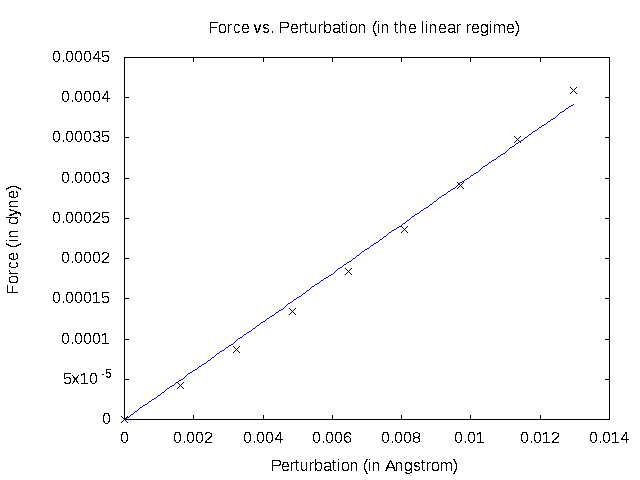
\includegraphics[scale=1.0]{data_engn.png}
    \caption{F vs displacement curve along Si <111> direction}
    \label{FvsD}
  \end{figure}
\end{center}
Note that in the calculation, the effective mass is 
\end{document}

